\section{Approach}

There are many considerations to take before creating a tool that should pretend
to understand the implementation of hardware and the implications of features
regarding energy efficiency. Care must be taken so that as much important
information as possible is extracted from the hardware model, concurrent, as
much noise and irrelevant information as possible must be filtered out.

\subsection{Energy Modelling}

While HDL-languages as well as computer architecture simulators have been around
for quite some time, energy estimation techniques is a more recent necessity.
Song et. al \cite{song2012instruction} identifies three major approaches to
processor power modelling used in the past, and introduces an instruction-based
energy estimation model that can be used for energy simulation at high speed.
Their proposed method is expressed through the following equation and includes
the desired features of past energy models.

\[
    P_{core}(t) = \frac{E_{unit} \cdot A_{datapath} \cdot w(t) +
    E_{static}}{T_{sampling}}
\]

This method depends on two things. First, one must know sufficient details of
the processor to identify datapath components in order to form the
$A_{datapath}$ matrix. Secondly, the energy unit vector $E_{unit}$ requires
circuit-level knowledge of the target processor. The former information can
often be found by reverse engineering and benchmarking, however, the latter is
rarely available for commercial processors. When building the model for PET, we
simplify the model from \cite{song2012instruction} by combining $A_{datapath}$
and $E_{unit}$ to form a vector of weights that directly corresponds to the cost
of an event. We can then model energy by the following formula.

\[
    P_{core}(t) = \frac{C \cdot w(t) + E_{static}}{T_{sampling}}
\]

Here, C represents the global cost vector -- a matrix enumerating the cost
for all event types. Please note that it is global and do not depend on time.

\subsection{Power Consuming Events}
\label{subsec:powerevents}

Choosing which events should be tracked and what workload that would give good
metrics is an important part of our method. We account for two main groups of
events; CPU instruction events and memory activity events. The contents of these
groups are listed in \autoref{tbl:events}. It is desirable to estimate energy
consumption on literally all types of computing systems, ranging from large-size
clusters to embedded systems. To provide this flexibility it was decided that
PET should parse log files from the simulators rather than being built-in on a
chosen simulator. Most active and working architectural simulators supports this
sort of trace logs, and even if they are formatted different, the effort of
adjusting to a new format is a lot less than the effort of building this tool
within even another simulator.

The trace logs contains information about everything that goes on within the
fictional computer, and thus PET can extract useful information from this log
file. A piece of such useful information is defined in PET at a \emph{simulator
event}. A simulator event can be thought of as a unit of work that uses a
specified amount of energy. When PET finds such an event, it increases the
modelled energy consumption along the timeline at the time the event took place.

\begin{table}[ht]
    \centering
    \begin{minipage}[b]{\linewidth}
        \centering
        \begin{tabular}{|l|l|}
            \hline
            IntAlu    & Integer basic ALU operation\\
            \hline
            IntMult    & Integer multiply ALU operation \\
            \hline
            MemRead    & Memory Read issued, triggers LS-unit \\
            \hline
            MemWrite    & Memory Write issued, triggeres LS-unit \\
            \hline
            SimdFloatMisc     & NEON-unit activated \\
            \hline
        \end{tabular}
        \subcaption{CPU Core Events}
    \end{minipage}

    \begin{minipage}[b]{\linewidth}
        \centering
        \begin{tabular}{|l|l|}
            \hline
            L1IR    & L1 instruction cache, read \\
            \hline
            L1IW    & L1 instruction cache, write \\
            \hline
            L1DR    & L1 data cache, read \\
            \hline
            L1DW    & L1 data cache, write \\
            \hline
            L2R     & L2 cache, read \\
            \hline
            L2W     & L2 cache, write \\
            \hline
            PhysR   & Main memory, read \\
            \hline
            PhysW   & Main memory, write \\
            \hline
        \end{tabular}
        \subcaption{Memory Events}
    \end{minipage}
    \caption{Power Consuming Events}
    \label{tbl:events}
\end{table}

The events briefly described in \autoref{tbl:events} are the ones recognized by
PET.  These events are selected based mainly on what information that is easily
extracted from a gem5-formatted trace log, but also adjusted by what information
we could check with performance counters without a very high amount of effort.
Most of this information is available from \cite{rundehvatum2013exploring},
where different instruction loops where measured with both ammeter and
performance counters. This is then correlated with \autoref{fig:a9arch} which
gives an architectural overview of the CPU core where different parts of the
pipeline is visible.

\begin{figure}
    \centering
    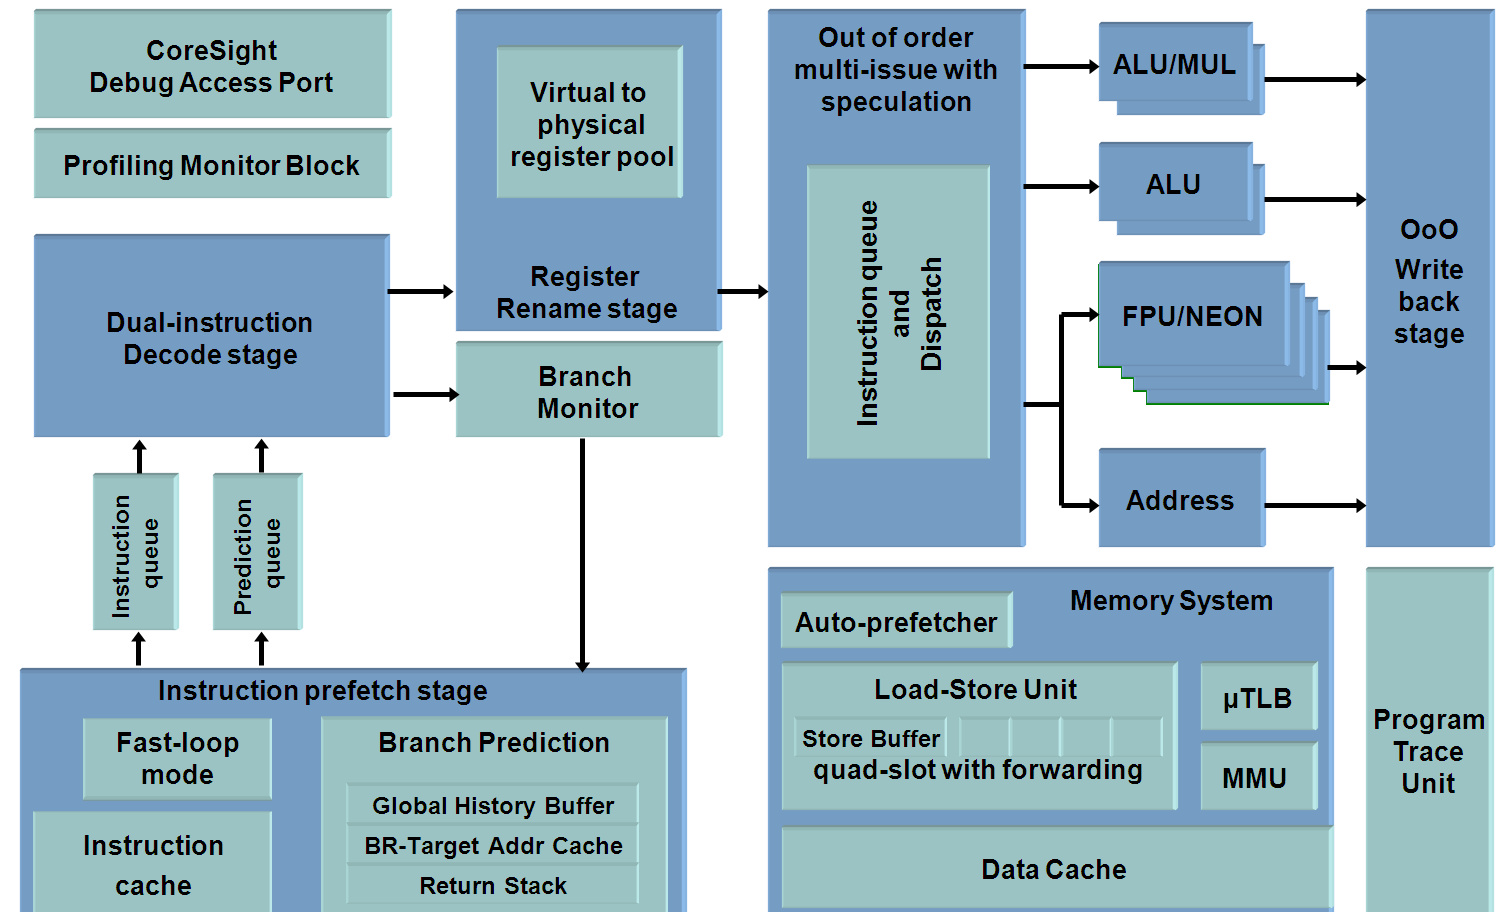
\includegraphics[width=\textwidth]{figs/A9-Pipeline-hres.jpg}
    \caption{A brief overview of the Cortex A9 Pipeline, figure from the ARM Cortex-A9 Whitepaper \cite{a9whitepaper}}
    \label{fig:a9arch}
\end{figure}
